\documentclass{article}

\usepackage{graphicx}
\usepackage{tikz}
\usepackage{tikzsymbols}
\usetikzlibrary{calc,patterns,shapes.geometric}
\pagestyle{empty}
\usepackage[margin=0pt]{geometry}
\geometry{papersize={14in,12in}}

\def\centerarc[#1](#2)(#3:#4:#5){\draw[#1] ($(#2)+({#5*cos(#3)},{#5*sin(#3)})$) arc (#3:#4:#5);}

\begin{document}
	\begin{figure}
		\centering
		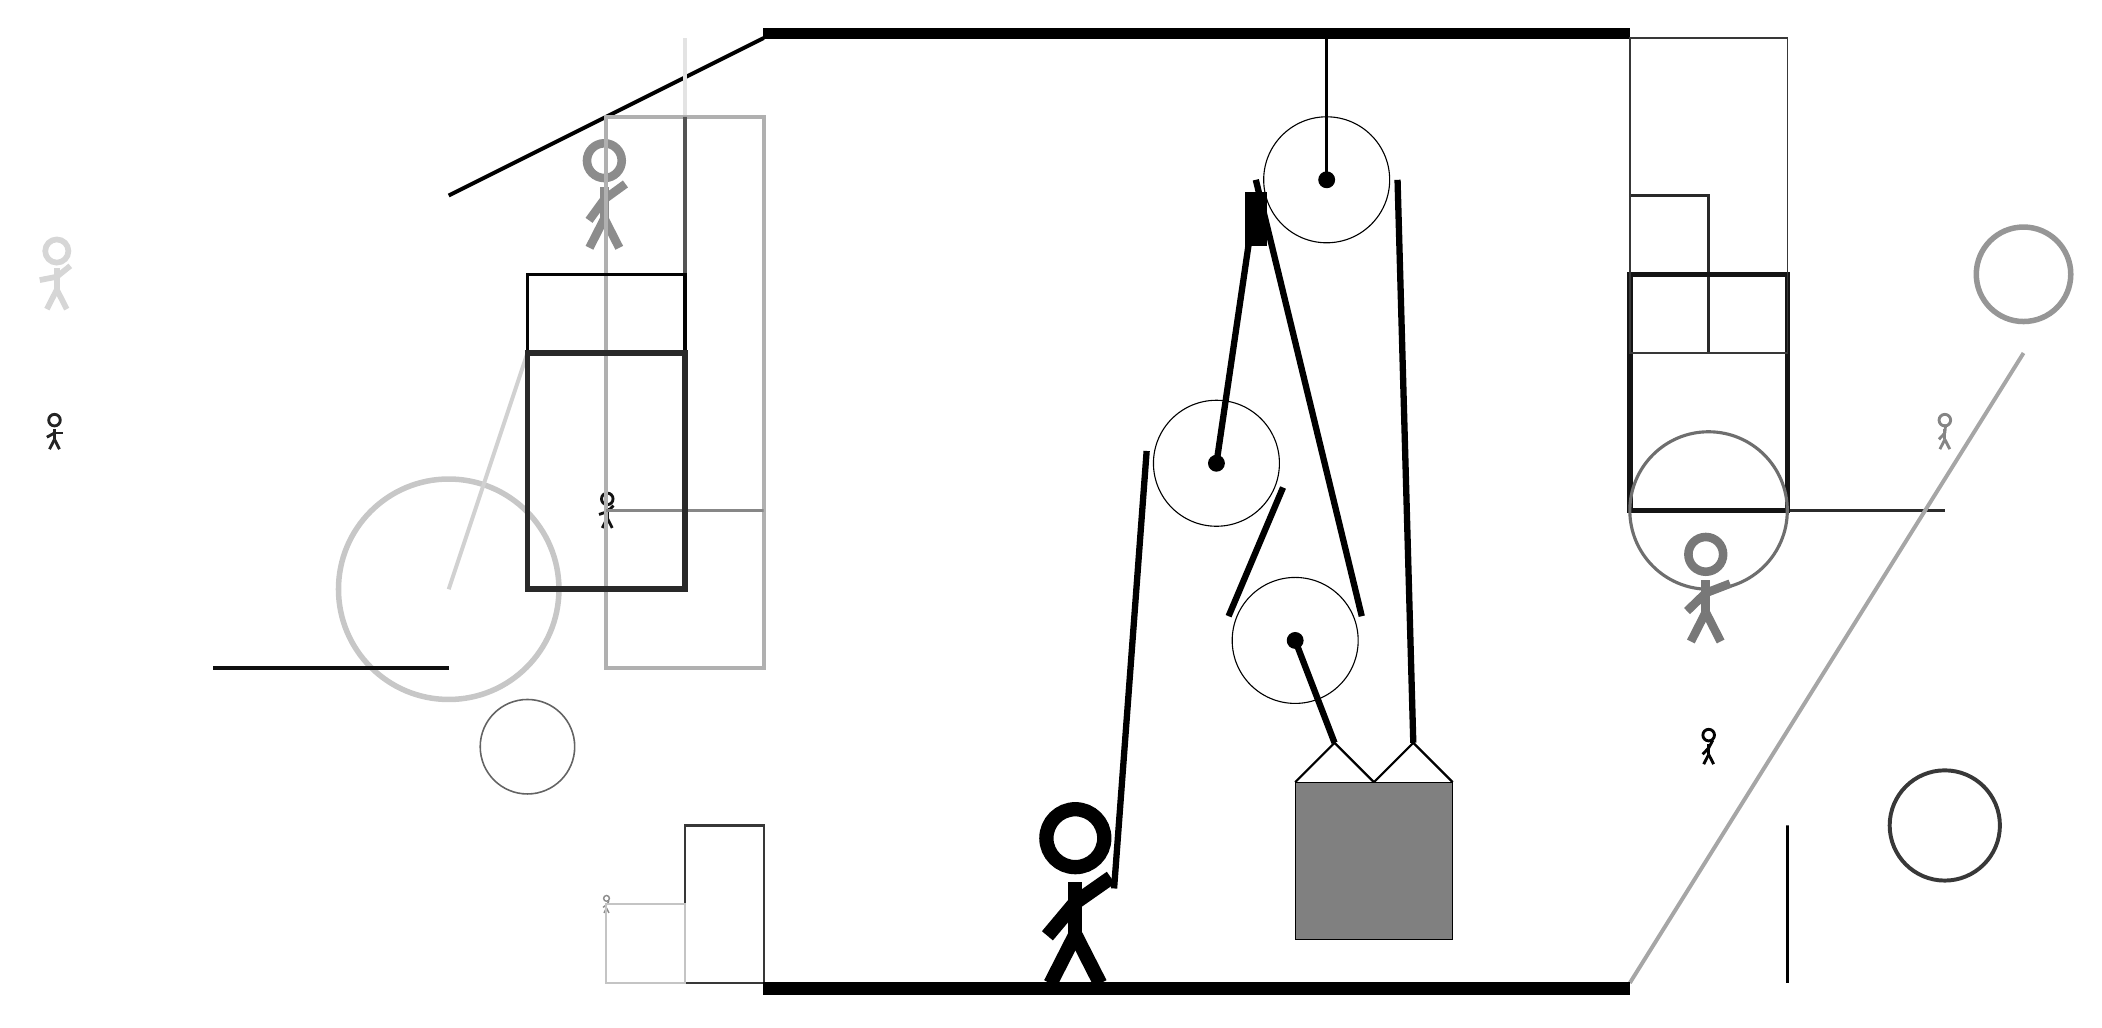
\begin{tikzpicture}
			%%%%% START %%%%%
			
			\draw[fill=black] (-6, 9) rectangle (5, 9.125);
			
			\draw (-0.25, 3.6) circle (0.8);
			\draw[fill=black] (-0.25, 3.6) circle (0.1);
			
			\draw (0.75, 1.35) circle (0.8);
			\draw[fill=black] (0.75, 1.35) circle (0.1);
			
			\node[line width=0.2mm, color=black!45] at (-8, 7) {\Strichmaxerl[6][54][36]};
			
			\draw[line width=0.5mm, color=black!100](-10, 7) -- (-6, 9);
			\draw [line width=0.7mm, color=black!22](-10, 2) circle (1.4);
			\draw[line width=0.3mm, color=black!100] (7, -3) rectangle (7, -1);
			\draw[line width=0.5mm, color=black!83](6, 3) -- (9, 3);
			\draw[line width=0.3mm, color=black!84] (5, 7) rectangle (6, 5);
			
			\draw[line width=0.5mm, color=black!18](-9, 5) -- (-10, 2);
			
			\draw[line width=0.5mm, color=black!11](-7, 9) -- (-7, 5);
			\draw[line width=0.7mm, color=black!92] (5, 3) rectangle (7, 6);
			
			\node[line width=0.7mm, color=black!93] at (-8, 3) {\Strichmaxerl[2][18][45]};
			
			\draw[line width=0.5mm, color=black!94](-10, 1) -- (-13, 1);
			\draw [line width=0.4mm, color=black!57](6, 3) circle (1.0);
			\draw[line width=0.5mm, color=black!31] (-6, 8) rectangle (-8, 1);
			
			\draw[line width=0.4mm, color=black!67] (-7, 8) rectangle (-7, 5);
			\draw[line width=0.5mm, color=black!35](10, 5) -- (5, -3);
			\node[line width=0.2mm, color=black!16] at (-15, 6) {\Strichmaxerl[4][11][39]};
			
			\draw [line width=0.2mm, color=black!61](-9, 0) circle (0.6);
			
			\draw[line width=0.5mm, color=black!47] (-6, 3) rectangle (-8, 3);
			\draw[line width=0.3mm, color=black!78] (-7, -1) rectangle (-6, -3);
			\draw[line width=0.4mm, color=black!99] (-7, 2) rectangle (-9, 6);
			\node[line width=0.5mm, color=black!45] at (-8, -2) {\Strichmaxerl[1][36][56]};
			
			\draw[line width=0.2mm, color=black!23] (-8, -2) rectangle (-7, -3);
			
			\node[line width=0.6mm, color=black!53] at (6, 2) {\Strichmaxerl[6][44][21]};
			\draw [line width=0.7mm, color=black!41](10, 6) circle (0.6);
			\draw[line width=0.2mm, color=black!78] (7, 5) rectangle (5, 9);
			
			\node[line width=0.2mm, color=black!99] at (6, 0) {\Strichmaxerl[2][46][62]};
			\node[line width=0.7mm, color=black!48] at (9, 4) {\Strichmaxerl[2][47][85]};
			\node[line width=0.7mm, color=black!86] at (-15, 4) {\Strichmaxerl[2][29][0]};
			
			\draw[line width=0.7mm, color=black!84] (-7, 5) rectangle (-9, 2);
			
			\draw [line width=0.5mm, color=black!78](9, -1) circle (0.7);
			
			\draw (1.15, 7.2) circle (0.8);
			\draw[fill=black] (1.15, 7.2) circle (0.1);
			\draw[very thick] (1.15, 7.2) -- (1.15, 9);
			
			\draw[thick]  (0.75, -0.45) -- (1.25, 0.05) -- (1.75, -0.45) -- (2.25, 0.05) -- (2.75, -0.45);
			\draw[fill=black!50] (0.75, -0.45) rectangle (2.75, -2.45);
			
			\draw[line width=0.8mm] (-0.25, 3.6) -- (0.25, 7.0);
			\draw[line width=0.8mm, fill=black](0.15, 6.4) rectangle (0.35, 7.0);
			\draw[line width=0.8mm] (-1.55, -1.8) -- (-1.1363, 3.7562);
			\centerarc[line width=0.8mm](-0.25, 3.6)(-20:170:0.9);
			\draw[line width=0.8mm] (0.5957, 3.2922) -- (-0.0957, 1.6578);
			\centerarc[line width=0.8mm](0.75, 1.35)(160:380:0.9);
			\draw[line width=0.8mm] (1.5957, 1.6578) -- (0.25, 7.2);
			\draw[line width=0.8mm](0.75, 1.35) -- (1.25, 0.05);
			\centerarc[line width=0.8mm](1.15, 7.2)(0:180:0.9);
			\draw[line width=0.8mm] (2.05, 7.2) -- (2.25, 0.05);
			
			\node at (-2, -1.9) {\Strichmaxerl[10][50][35]};
			
			\draw[fill=black] (-6, -3) rectangle (5, -3.15);
			
			%%%%% END %%%%%
		\end{tikzpicture}
	\end{figure}	
\end{document}